\documentclass{article}
\usepackage[left=0.5in,top=0.5in,right=0.5in,bottom=0.5in]{geometry}
\usepackage[dvipsnames]{xcolor}
\usepackage[english]{babel}
\usepackage[utf8]{inputenc}
\usepackage{subcaption}
\usepackage{graphicx}
\usepackage{
  amssymb,
  amsmath,
  amsthm,
  latexsym
}
\graphicspath{{./images/}}
\title{Moth Evolution Simulation Lab Report}
\author{Philip Kim}
\date{\today}
\begin{document}
\maketitle
\begin{enumerate}
  \item After the conclusion of this simulation, log your results. Start this by attaching a screenshot of your graph. In which direction did the allele frequencies change?
  \begin{figure}[h!]
    \begin{center}
      \begin{subfigure}[b]{0.7\textwidth}
        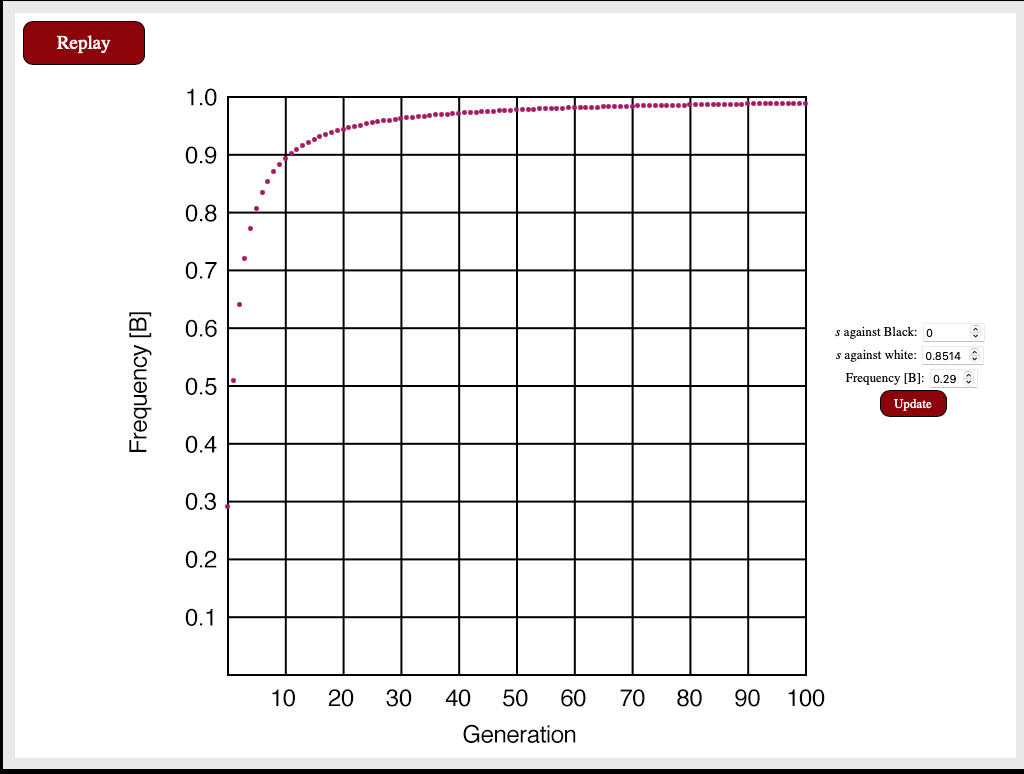
\includegraphics[width=\textwidth]{white.png}
      \end{subfigure}
      \caption*{Initial frequency of allele \textbf{B}: 0.29}
    \end{center}
  \end{figure}
  \begin{itemize}
    \item The frequency of the black allele increased to 1.0, or 100\% after 100 generations which means the darker moths became the most frequent in the population. Also, the selection coefficient against white is much higher than the selection coefficient against black since it was easier to spot the light-colored moths.
  \end{itemize}
  \item Explain the mechanism by which these changes occurred. What is this mechanism called?
  \begin{itemize}
    \item Population of peppered moths live in the woods near industrial cities where pollution has darkened the tree trunks. Due to natural genetic variation, some moths have light-colored wings flecked with scattered dark sports and other moths with solid black wings. Light-colored moths are more visible to their predators than the black moths. Thus, light-colored moths are eaten at a higher frequency compared to the black moths. Since the black moths have a higher survival rate, they are more likely to have offsprings with black colored wings, which results in a higher fraction of black moths for the next generation.
    \item The process whereby individuals better adapted to their environments tend to better survive and reproduce, changing the genetic makeup of populations over time is known as evolution by \textbf{natural selection}.
  \end{itemize}
  \item Which of the three genotypes do you think would be most fit in a rural area, far from cities, such as the woods in the far South of England?
  \begin{itemize}
    \item Genotype \textbf{bb} would best fit in an rural environment in the woods as far away from industrial pollution. Without the environment effecting microevolution and natural selection, peppered moths with light-colored wings flecked and scattered dark spots would rest on lichen-encrusted tree trunks which made it very difficult for predators to spot. Therefore, these light-colored moths would evolve by natural selection.
  \end{itemize}
  \item Which of the three genotypes do you think would be most fit in the woods near industrial cities?
  \begin{itemize}
    \item Genotype \textbf{BB} and \textbf{Bb} would best fit in an urban environment in the woods that has industrial pollution would darken the tree trunks which made it very difficult for predators to spot the dark moths. Therefore, these dark-colored moths would evolve by natural selection.
  \end{itemize}
  \item What do you think happened after England passed clean air laws?
  \begin{itemize}
    \item After England passed clean air laws and if the trees changed its color from dark to a lighter color then you could expect the moths with light-colored wings evolve by natural selection. However, if the trees remained dark then the frequency of the \textbf{B} allele value would be higher than \textbf{b} allele.
  \end{itemize}
  \item Play around with the simulation and change the ``selection against Black, selection against White.'' What do you notice?
  \begin{itemize}
    \item After changing ``\textbf{s against white}'' from 0.8514 to 0 and ``\textbf{s against black}'' from 0 to 0.8514, there is almost an inverse relationship. Initially, more black moths would evolve through natural selection and after the change in selection coefficient more white moths would evolve through natural selection.
  \end{itemize}
\end{enumerate}
\end{document}